% !Mode:: "TeX:UTF-8"
% !TEX program  = xelatex
\documentclass[a4paper]{article}
\usepackage{amsmath}
\usepackage{amssymb}
\usepackage{ctex}
\usepackage{subfig}
%\usepackage{braket}
%\usepackage[european]{circuitikz}
\usepackage{multirow}
\usepackage{float}
\usepackage{graphicx}
\usepackage{geometry}
\usepackage{bm}
\geometry{left=2.5cm,right=2.5cm,bottom=2.5cm,top=2.5cm}
\title{近代物理实验:半导体的霍尔系数与电导率测量}
\author{ 姓名\quad 学号\quad 匡亚明学院}
\date{}
\begin{document}
	\maketitle
	\bibliographystyle{unsrt}
	%--------main-body------------
	
\section{引言}
1879年,霍尔(E.H.Hall)研究通有电流的导体在磁场中受力时,发现在垂直于磁场和电流的方向上产生了电动势,这个电磁效应称为“霍尔效应”。在半导体材料中,霍尔效应比在金属中大几个数量级,引起人们对它的深入研究。霍尔效应的研究在半导体理论的发展中起了重要的推动作用。直到现在,霍尔效应的测量仍是研究半导体性质的重要实验方法。利用霍尔系数和电导率的联合测晕,可以用来研究半导体的导电机构(本征导电和杂质导电)、散射机构(晶格散射和杂质散射),并可以确定半导体的一些基本参数,如:半导体材料的导电类型、载流子浓度、迁移率大小、禁带宽度、杂质电离能等。利用霍尔效应制成的元件,称为霍尔元件,也已广泛地用千测试仪器和自动控制系统中。

\section{实验目的}
\begin{enumerate}
	\item 了解半导体中霍尔效应的产生原理,霍尔系数表达式的推导及其副效应的产生和消除。
	\item 掌握霍尔系数和电导率的测量方法。通过测量数据处理判别样品的导电类型,计算载流子浓度、电导率、霍尔迁移率,并求出材料的禁带宽度。
\end{enumerate}

\section{实验原理}
\subsection{霍尔效应和霍尔系数}
设一块半导体的$x$方向上有均匀的电流$I_x$流过,在$z$方向上加有磁场$B_z$,则在这块半导体的$y$方向上出现一横向电势差$U_H$,这种现象被称为“霍尔效应”,$U_H$称为“霍尔电压”,所对应的横向电场$E_H$称为“霍尔电场”,见图(\ref{fig1})。
\begin{figure}[!h]
	\centering
	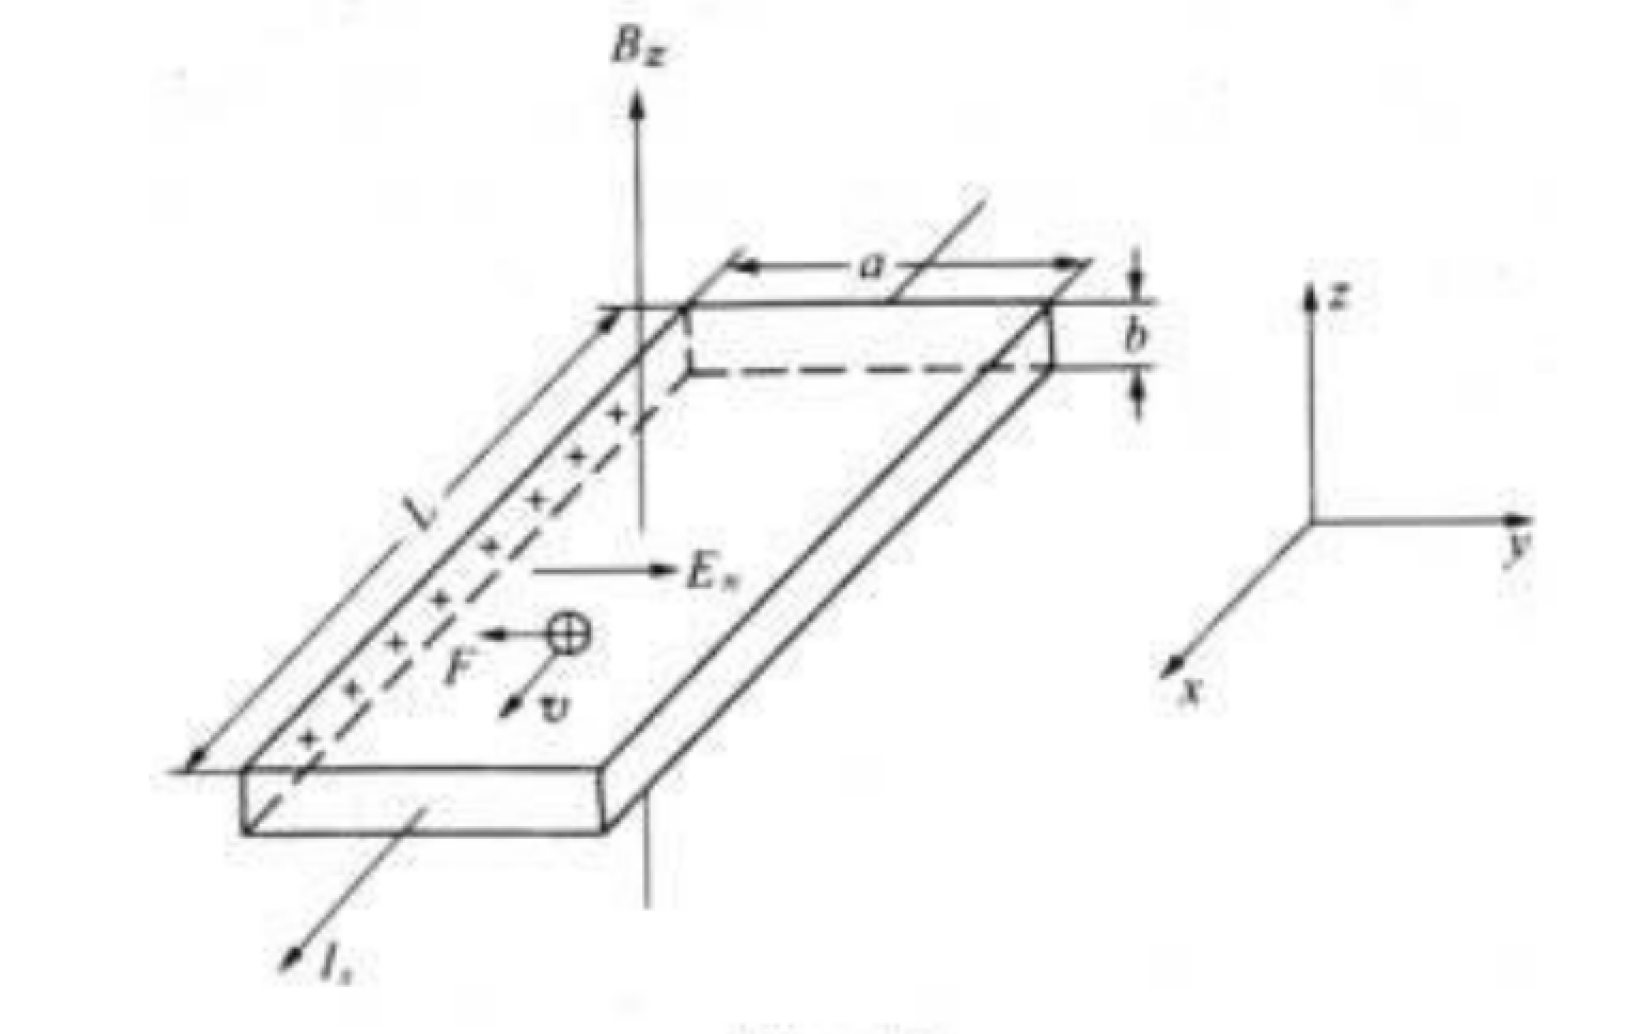
\includegraphics[width=6cm]{fig/fig1.png}\\
	\caption{霍尔效应示意图}\label{fig1}
\end{figure}

实验指出,霍尔电场强度$E_H$的大小与流经样品的电流密度$J_x$和磁感应强度$B_z$的乘积成正比
\begin{equation}\label{6.1.1}
E_H=R_H \cdot J_x \cdot B_z 
\end{equation}
式中比例系数$R_H$称为“霍尔系数”。

下面以p型半导体样品为例,讨霍论尔效应的产生原理并推导、分析霍尔系数的表达式。

半导体样品的长、宽、厚分别为$L$、$a$、$b$,半导体载流子(空穴)的浓度为$p$,它们在电场$E_x$作用下,以平均漂移速度$v_x$沿$x$方向运动,形成电流$I_x$,在垂直于电场$E_x$方向上加一磁场$B_z$,则运动着的载流子要受到洛仑兹力的作用
\begin{equation}\label{6.1.2}
\bm{F}=q\bm{v} \times \bm{B}
\end{equation}
式中$q$为空穴电荷电量。该洛仑兹力指向$-y$方向,因此载流子向$-y$方向偏转,这样在样品的左侧面就积累了空穴,从而产生了一个指向$+y$方向的电场——霍尔电场$\bm{E}_y$。当该电场对空穴的作用力$q E_y$与洛仑兹力相平衡时,空穴在$y$方向上所受的合力为零,达到稳态。稳态时电流仍沿$x$方向不变,但合成电场$\bm{E}=\bm{E}_x+\bm{E}_y$不再沿$x$方向,$\bm{E}$与$x$轴的夹角称“霍尔角”。在稳态时,有
\begin{equation}\label{6.1.3}
qE_y=qv_x B_z
\end{equation}
若$E_y$是均匀的,则在样品左、右两侧面间的电位差
\begin{equation}\label{6.1.4}
U_H=E_y\cdot a=v_x B_z a
\end{equation}
而$x$方向的电流强度
\begin{equation}\label{6.1.5}
I_x=q\cdot p\cdot v_x\cdot ab
\end{equation}
将式(\ref{6.1.5})的$v_x$代入式(\ref{6.1.4})得霍尔电压
\begin{equation}\label{6.1.6}
U_H=(\frac{1}{q\cdot p})\frac{I_x\cdot B_z}{b}
\end{equation}
由式(\ref{6.1.1})、(\ref{6.1.3})、(\ref{6.1.5})得霍尔系数
\begin{equation}\label{6.1.7}
R_H=\frac{1}{q\cdot p}
\end{equation}
对于n型样品,载流子(电子)浓度为$n$,霍尔系数为
\begin{equation}\label{6.1.8}
R_H=-\frac{1}{q\cdot p}
\end{equation}

上述模型过于简单。根据半导体输运理论,考虑到载流子速度的统计分布以及载流子在运动中受到散射等因素,在霍尔系数的表达式中还应引入一个霍尔因子$A$,则式(\ref{6.1.7})、(\ref{6.1.8})应修正为
\begin{equation}\label{6.1.9}
\text{p型:}R_H=A\cdot\frac{1}{q\cdot p}
\end{equation}
\begin{equation}\label{6.1.10}
\text{n型:}R_H=-A\cdot\frac{1}{q\cdot n}
\end{equation}
$A$的大小与散射机理及能带结构有关。由理论算得,在弱磁场条件下,对球形等能面的非简并半导体,在较高温度(此时,晶格散射起主要作用)情况下,
\begin{equation*}
A=\frac{3\pi}{8}=1.18
\end{equation*}
一般地,Si、Ge等常用半导体在室品下属于此种情况,$A$取为1.18。在较低温度(此时,电离杂质散射起主要作用)情况下,
\begin{equation*}
A=\frac{315\pi}{512}=1.93
\end{equation*}
对于高载流子浓度的简并半导体以及强磁场条件,$A=1$;对于晶格和电离杂质混合散射情况,一般取文献报道的实验值。

上面讨论的是只有电子或只有空穴导电的情况。对于电子、空穴混合导电的情况,在计算$R_H$时应同时考虑两种载流子在磁场下偏转的效果。对于球形等能面的半导体材料,可以证明:
\begin{equation}\label{6.1.11}
R_H=\frac{A(p\mu_p^2-n\mu_n^2)}{q(p\mu_p+n\mu_n)^2}=\frac{A(p-nb^2)}{q(p+nb)^2}
\end{equation}
式中$b=\mu_n/\mu_p$;$\mu_n$、$\mu_p$为电子和空穴的迁移率。

从霍尔系数的表达式可以看出:由$R_H$的符号(也即$U_H$的符号)可以判断载流子的类型,正为p型,负为n型(注意,所谓正、负是指在$xyz$坐标系中相对千$y$轴方向而言,见图(\ref{fig1})。$l$、$B$的正方向分别为$x$轴、$z$轴的正方向,则霍尔电场方向为$y$轴方向。当霍尔电场方向的指向与$y$正向相同时,则$U_H$为正。);$R_H$的大小可确定载流子的浓度;还可以结合测得的电导率$\sigma$算出如下定义的“霍尔迁移率”$\mu_H$
\begin{equation}\label{6.1.12}
\mu_H=|R_H|\cdot \sigma
\end{equation}
$\mu_H$的量纲与载流子的迁移率相同,通常为cm$^2$/V$\cdot$s(厘米$^2$/伏$\cdot$秒),它的大小与载流子的“漂移(或电导)迁移率”有密切的关系。

霍尔系数$R_H$可以在实验中测量出来,若采用国际单位制,由式(\ref{6.1.6})、(\ref{6.1.7})可得
\begin{equation}\label{6.1.13}
R_H=\frac{U_H \cdot b}{I_x \cdot B_z}(\text{m}^3/\text{C})
\end{equation}
但在半导体学科中习惯采用实用单位制(其中,$b$:厘米,$B_z$:高斯G),则
\begin{equation*}
R_H=\frac{U_H \cdot b}{I_x \cdot B_z}\times 10^8(\text{cm}^3/\text{C})
\end{equation*}

\subsection{霍尔系数与温度的关系}
$R_H$与载流子浓度之间有反比关系,因此当温度不变时,$R_H$不会变化;而当温度改变时,载流子浓度发生变化,$R_H$也随之变化。图是$R_H$随温度$T$变化的关系图。图中纵坐标为$R_H$的绝对值,曲线A、B分别表示n型和p型半导体的霍尔系数随温度的变化曲线。
\begin{figure}[!h]
	\centering
	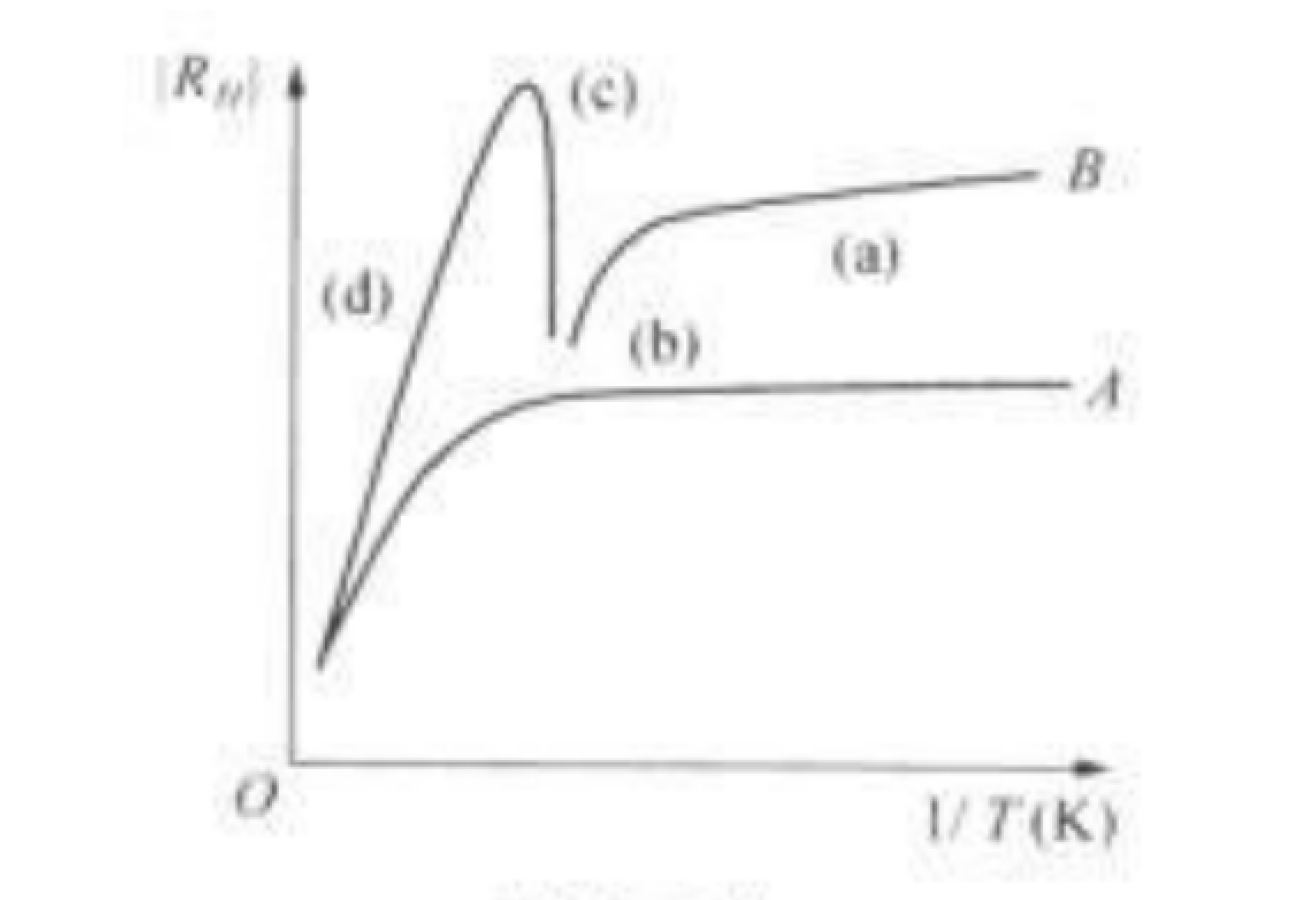
\includegraphics[width=6cm]{fig/fig2.png}\\
	\caption{霍尔系数随温度变化曲线}\label{fig2}
\end{figure}

下面简要地讨论曲线B:
\begin{enumerate}
\item 杂质电离饱和区。在曲线(a)段,所有的杂质都已电离,载流子浓度保待不变。p型半导体中$p\gg N$,式(\ref{6.1.11})中$nb^2$可忽略,可简化为
\begin{equation*}
R_H=A\cdot\frac{1}{q p}=A\cdot\frac{1}{q N_A}>0
\end{equation*}
式中$N_A$为受主杂质浓度。
\item 温度逐渐升高,价带上的电子开始激发到导带,由于$\mu_n>\mu_p$,所以$b>1$,当温度升到使$p = nb^2$时,$RH=0$,出现了图中(b)段。
\item 温度再升高时,更多的电子从价带激发到导带,$p<nb^2$而使$R_H<0$,式(\ref{6.1.11})中分母增大,$R_H$减小,将会达到一个负的极值(图中(c)点)。此时价带的空穴数$p=n+N_A$,将它代入式(\ref{6.1.11}),并对$n$求微商,可以得到当$n=N_A/(b-1)$时,$R_H$达到极值$R_{HM}$:
\begin{equation}\label{6.1.14}
R_{HM}=-\frac{A}{qN_A}\cdot \frac{(b-1)^2}{4b}
\end{equation}
由此式可见,当测得$R_{HM}$和杂质电离饱和区的$R_H$,就可定出$b$的大小。
\item 当温度继续升高,达本征范围时,半导体中载流子浓度大大超过受主杂质浓度,所以$R_H$随温度上升而呈指数下降,$R_H$只由本征载流子浓度$n_i$来决定,此时杂质含量不同或杂质类型不同的曲线都将趋聚在一起,见图中(d)段。
\end{enumerate}

\subsection{半导体的电导率}
在半导体中若有两种载流子同时存在,则其电导率$\sigma$为
\begin{equation}\label{6.1.15}
\sigma=qp\mu_p+qn\mu_n
\end{equation}

实验得出$\sigma$与温度$T$的关系曲线如图。
\begin{figure}[!h]
	\centering
	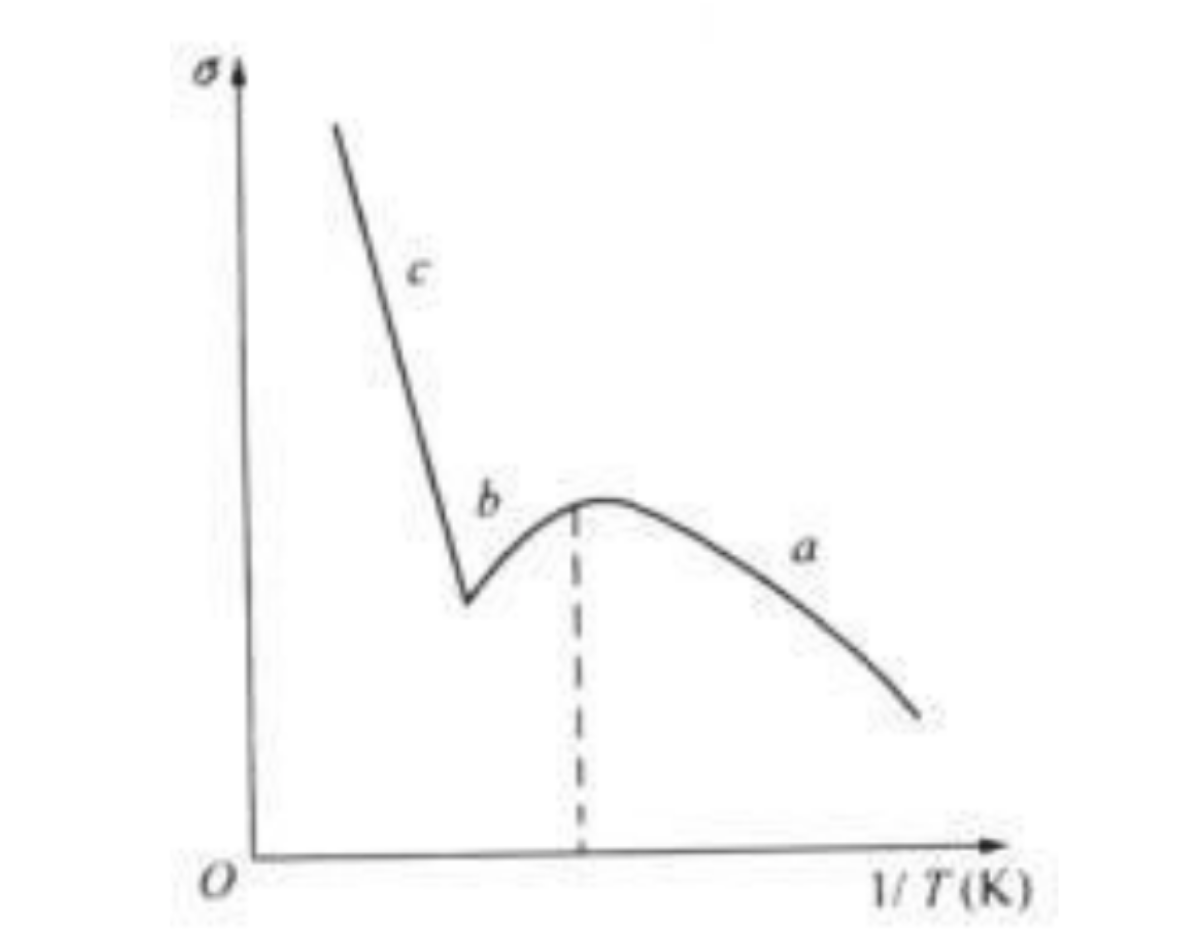
\includegraphics[width=6cm]{fig/fig3.png}\\
	\caption{$\sigma$与温度$T$关系曲线}\label{fig3}
\end{figure}

现以p 型半导体为例分析:
\begin{enumerate}
\item 低温区。在低温区杂质部分电离,杂质电离产生的载流子浓度随温度升高而增加,而且$\mu_p$在低温下主要取决于杂质散射,它也随温度升高而增加。因此,$\sigma$随$T$的增加而增加,见图的a段。
\item 室温附近。此时,杂质已全部电离,载流子浓度基本不变,这时晶格散射起主要作用,使$\mu_p$随$T$的升高而下降,导致$\sigma$随$T$的升高而下降,见图的b段。
\item 高温区。在这区域中,本征激发产生的载流子浓度随温度升高而指数地剧增,远远超过$\mu_p$的下降作用,致使$\sigma$随$T$而迅速增加,见图的c段。
\end{enumerate}

在本征激发区,本征激发产生的电子浓度近似等于空穴浓度,且远远超过杂质离化产生的载流子浓度,有$p\approx n$,载流子浓度 $n$与$T$、$E_g$有以下关系:
\begin{equation*}
n\propto T^{\frac{3}{2}} \exp(-\frac{E_g}{2kT})
\end{equation*}
式中$E_g$为禁带宽度,$k$为波尔兹曼常数,$T$为绝对温度。此时$\sigma=qn(\mu_n+\mu_p)$,由于迁移率与$T^{-3/2}$成正比,所以$\ln\sigma$与$E_g/2kT$成正比。因此在本征激发范围,由$\ln\sigma \sim 1/T$曲线的斜率可以算出样品材料的禁带宽度。

实验中电导率$\sigma$可由
\begin{equation}\label{6.1.16}
\sigma=\frac{1}{\rho}=\frac{I\cdot l}{U_\sigma \cdot ab}
\end{equation}
式中$\rho$为电阻率,$I$为流过样品的电流,$U_\sigma$、$l$分别为两测量点间的电压降和长度。

对于不规则形状的半导体样品,常用范德堡(Van der Pauw)法测量,它对电极对称性的要求较低,在半导体新材料的研究中用得较多。

\subsection{霍尔效应中的副效应及其去除}
霍尔系数的测量通常伴随一些热磁副效应、电极不对称等因素引起的附加电压叠加在霍尔电压$U_H$上,下面作些简要说明:
\begin{enumerate}
\item 爱廷豪森(Ettinghausen)效应。在样品$x$方向通电流$I_x$,由于载流子速度分布的统计性,大于和小于平均速度的载流子在洛仑兹力和霍尔电场力的作用下,沿y 轴的相反两侧偏转,其动能将转化为热能,使两侧产生温差。由于电极和样品不是同一种材料,电极和样品形成热电偶,这一温差将产生温差电动势$U_E$,而且有
$$U_E\propto I_x \cdot B_z$$
这就是爱廷豪森效应。$U_E$方向与电流$I$及磁场$B$的方向有关。
\item 能斯脱(Nernst)效应。如果在$x$方向存在热流$Q_x$(往往由于$x$方向通以电流,两端电极与样品的接触电阻不同而产生不同的焦耳热,致使$x$方向两端温度不同),沿温度梯度方向扩散的载流子将受到$B_z$作用而偏转,在$y$方向上建立电势差$U_N$,有
$$U_N \propto Q_x \cdot B_z$$
这就是能斯脱效应。$U_N$方向只与$B$方向有关。
\item 里纪-勒杜克(Righi-Ledue)效应。当有热流$Q_x$沿$x$方向流过样品,载流子将倾向于由热端扩散到冷端,与爱廷豪森效应相仿,在$y$方向产生温差,这温差将产生温差电势$U_{RL}$,这一效应称里纪-勒杜克效应。
$$U_{RL} \propto Q_x \cdot B_z$$
$U_{RL}$的方向只与$B$的方向有关。
\item 电极位置不对称产生的电压降$U_0$。在制备霍尔样品时,$y$方向的测量电极很难做到处于理想的等位面上,见图(\ref{fig4})。即使在未加磁场时,在A、B两电极间也存在一个由于不等位电势引起的欧姆压降$U_0$:
$$U_0= I_x \cdot R_0$$
其中$R_0$为A、B两电极所在的两等位面之间的电阻,$U_0$方向只与$I_x$方向有关。
\begin{figure}[!h]
	\centering
	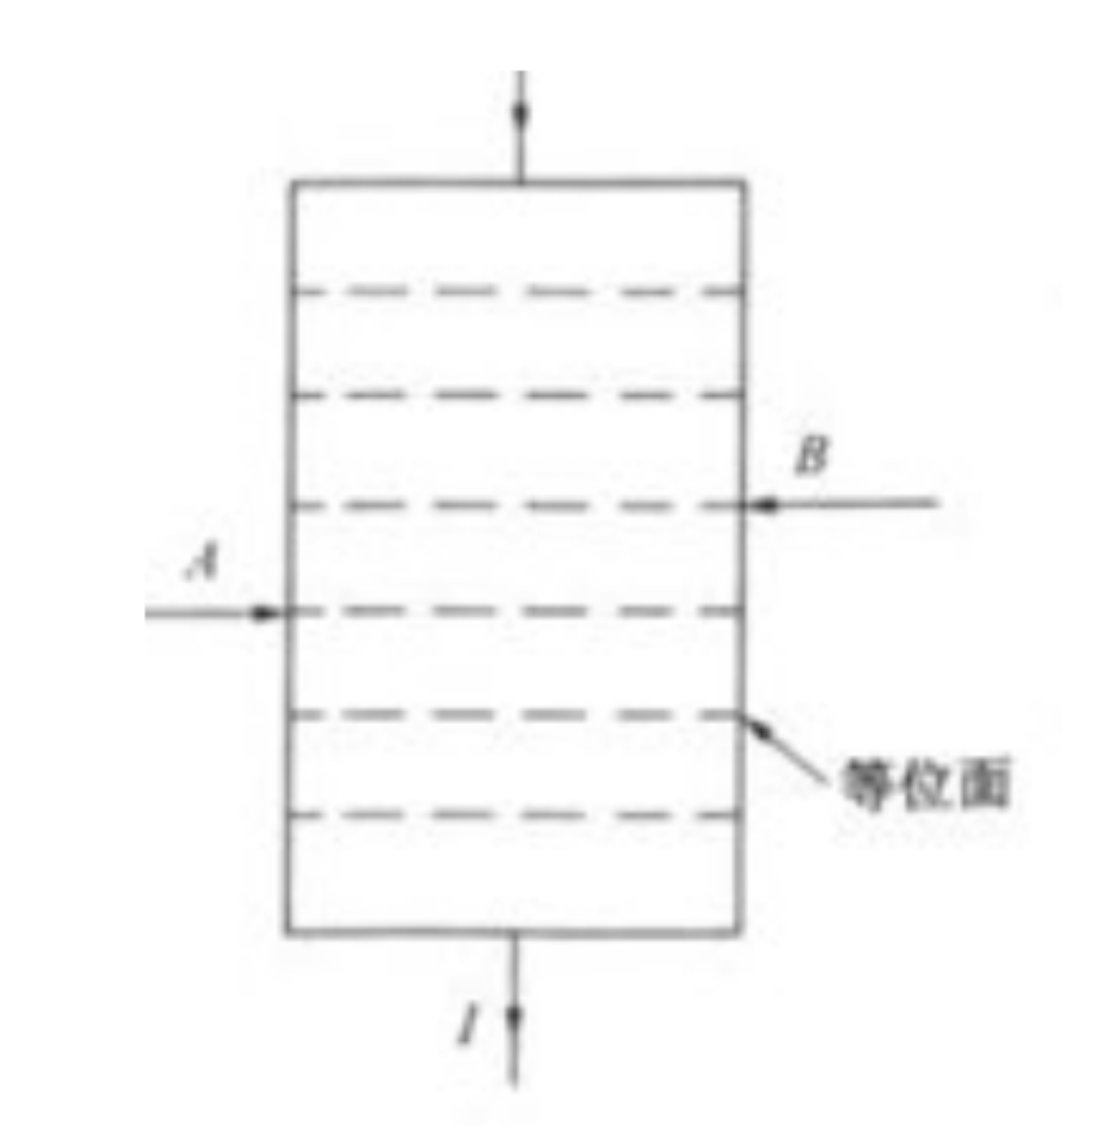
\includegraphics[width=4cm]{fig/fig4.png}\\
	\caption{等位面示意图}\label{fig4}
\end{figure}
\item 样品所在空间如果沿$y$方向有温度梯度,则在此方向上产生的温差电势$U_T$也将叠加在$U_H$中,$U_T$与$I$、$B$方向无关。
\end{enumerate}

要消除上述诸效应带来的误差,应改变$I$和$B$的方向,使$U_N$、$U_{RL}$、$U_0$和$U_T$从计算结果中消除,然而$U_E$却因与$I$、$B$方向同步变化而无法消除,但$U_E$引起的误差很小,可以忽略。

实验时在样品上加磁场$B$和通电流$I$,则$y$方向两电极间产生电位差$U$,自行定义磁场和电流的正方向改变磁场和电流方向,测出四组数据:

加$+B$、$+I$时,$U_1=+U_H+U_E+U_N+U_{RL}+U_0+U_T$

加$+B$、$-I$时,$U_2=-U_H-U_E+U_N+U_{RL}-U_0+U_T$

加$-B$、$-I$时,$U_3=+U_H+U_E-U_N-U_{RL}-U_0+U_T$

加$-B$、$+I$时,$U_4=-U_H-U_E-U_N-U_{RL}+U_0+U_T$\\
由以上四式可得
\begin{equation}\label{6.1.17}
U_H+U_E\approx U_H=\frac{U_1-U_2+U_3-U_4}{4}
\end{equation}
将实验时测得的$U_1$、$U_2$、$U_3$和$U_4$代入上式,就可消除$U_N$、$U_{RL}$、$U_0$和$U_T$等附加电压引入的误差,得到霍尔电压$U_H$。


\section{实验仪器}
\subsection{样品制备}
在霍尔系数的测量中样品的制备是一个重要环节,样品电极位置的对称性、电极接触电阻的大小以及对称性等都直接影响到测量结果。此外,为了避免两电流电极的少数载流子注入和短路作用对测星结果的影响,两个端面要磨毛,并做成长度比宽度及厚度大得多的矩形 样品。实验中把一定厚度的硅、绪单晶片或外延硅薄层(外延层和衬底的掺杂浓度不一样)样品采用切割或腐蚀方法做成矩(或桥)形样品,在电极处用蒸发、光刻、合金化等平面工艺技术制成欧姆接触电极。

\subsection{实验仪器}
实验仪器包括磁场、变温设备、测量线路、数字电压表等几个主要部分。

\section{实验内容}


\section{实验讨论}


\section{思考题}
\subsection{以n型半导体样品为例,说明如何确定霍尔电场的方向}

\subsection{叙述载流子迁移率(又称漂移迁移率或电导迁移率)的物理意义,并推出n型(或p型)半导体的漂移迁移率$\mu_n$ (或$\mu_p$)与霍尔迁移率$\mu_H$的关系式。}
\subsection{在杂质电离温区,载流子浓度可由式(\ref{6.1.9})或式(\ref{6.1.10})计算,当温度升高至本征激发开始后,出现p、n两种载流子,此时应如何从实验中求出载流子浓度?}

\end{document}
